\setcounter{chapter}{21}
\renewcommand{\thetheorem}{22.a.\arabic{theorem}}
\setcounter{theorem}{0}

\chapter{Euclidean and Hermitian Spaces}

\section{Euclidean and Hermitian (Unitary) spaces}

At last (!) we endow our spaces with a geometric structure. We work here with vector spaces $V$ over $K = \mathbb{R}$ or $K = \mathbb{C}$. Over $\mathbb{R}$ we will have Euclidean spaces. Over $\mathbb{C}$ we will have Hermitian (a.k.a.\ unitary) spaces.

% def 22.a.1
\begin{definition}[Scalar Product]
\label{def:scalar_product_real}
Let $V$ be a vector space over $\mathbb{R}$. A \newterm{scalar product} (a.k.a.\ inner product) is a function $V \times V \longrightarrow \mathbb{R}$, denoted by $v, w \mapsto \langle v, w \rangle$ (or $(v,w)$), that has the following properties:
\begin{enumerate}[label=\textbf{(\alph*)}]
    \item Linearity in the $1^{\text{st}}$ variable:
    \begin{align*}
        \langle v_1 + v_2, w \rangle &= \langle v_1, w \rangle + \langle v_2, w \rangle \quad \forall v_1, v_2, w \in V \\
        \langle \alpha v, w \rangle &= \alpha \langle v, w \rangle \quad \forall \alpha \in \mathbb{R}, \; v, w \in V.
    \end{align*}
    \item Linearity in the $2^{\text{nd}}$ variable:
    \begin{align*}
        \langle v, w_1 + w_2 \rangle &= \langle v, w_1 \rangle + \langle v, w_2 \rangle \quad \forall v, w_1, w_2 \in V \\
        \langle v, \alpha w \rangle &= \alpha \langle v, w \rangle \quad \forall \alpha \in \mathbb{R}, \; v, w \in V.
    \end{align*}
    \item Symmetry:
    \[
        \langle v, w \rangle = \langle w, v \rangle \quad \forall v, w \in V.
    \]
    \item Positivity:
    \[
        \forall 0 \neq v \in V, \quad \langle v, v \rangle > 0.
    \]
\end{enumerate}
We call $(V, \langle \cdot, \cdot \rangle)$ a \newterm{Euclidean space}, or a space endowed with a scalar product.
\end{definition}

% def 22.a.2
\begin{definition}[Hermitian Product]
\label{def:hermitian_product_complex}
Let $V$ be a vector space over $\mathbb{C}$. A \newterm{Hermitian product} (or inner product) on $V$ is a function $V \times V \longrightarrow \mathbb{C}$, denoted by $v, w \mapsto \langle v, w \rangle$, with the following properties:
\begin{enumerate}[label=\textbf{(\alph*)}]
    \item Linearity in the $1^{\text{st}}$ variable:
    \begin{align*}
        \langle v_1 + v_2, w \rangle &= \langle v_1, w \rangle + \langle v_2, w \rangle \quad \forall v_1, v_2, w \in V \\
        \langle \alpha v, w \rangle &= \alpha \langle v, w \rangle \quad \forall \alpha \in \mathbb{C}, \; v, w \in V.
    \end{align*}
    \item Sesquilinearity (complex anti-linearity) in the $2^{\text{nd}}$ variable:
    \begin{align*}
        \langle v, w_1 + w_2 \rangle &= \langle v, w_1 \rangle + \langle v, w_2 \rangle \quad \forall v, w_1, w_2 \in V \\
        \langle v, \alpha w \rangle &= \overline{\alpha} \langle v, w \rangle \quad \forall \alpha \in \mathbb{C}, \; v, w \in V.
    \end{align*}
    \item Hermitian property:
    \[
        \langle v, w \rangle = \overline{\langle w, v \rangle} \quad \forall v, w \in V.
    \]
    \item Positivity:
    \[
        \forall 0 \neq v \in V, \quad \langle v, v \rangle > 0.
    \]
\end{enumerate}
We call $(V, \langle \cdot, \cdot \rangle)$ a \newterm{Hermitian} (or unitary) space.
\end{definition}

\begin{remark}
Recall that if $\alpha = a + ib \in \mathbb{C}$, where $a, b \in \mathbb{R}$ and $i = \sqrt{-1}$, then $\overline{\alpha} := a - ib$ is the complex conjugate of $\alpha$. Recall also that $\alpha \cdot \overline{\alpha} = a^2 + b^2 = |\alpha|^2 \geq 0$, with equality if and only if $\alpha = 0$.

The definition of a Hermitian product ``coincides'' with a scalar product if $V$ is over $\mathbb{R}$, and we allow $\alpha$ only in $\mathbb{R}$.
\end{remark}

% lemma 22.a.3
\begin{lemma}
\label{lem:basic_properties_inner_prod}
Let $V$ be a Euclidean/Hermitian vector space. Then:
\begin{enumerate}[label=\textbf{(\alph*)}]
    \item $\forall v \in V$, $\langle 0, v \rangle = \langle v, 0 \rangle = 0$.
    \item Let $w \in V$. If $\langle v, w \rangle = 0$ for all $v \in V$, then $w = 0$. \hfill (Exercise)
    \item Let $w_1, w_2 \in V$. If $\langle v, w_1 \rangle = \langle v, w_2 \rangle$ for all $v \in V$, then $w_1 = w_2$.
\end{enumerate}
\end{lemma}

% def 22.a.4
\begin{definition}
\label{def:norm_distance_orthogonality}
\begin{enumerate}[label=\textbf{(\alph*)}]
    \item Let $V$ be a Euclidean/Hermitian vector space. For all $v \in V$, define $\|v\| := \sqrt{\langle v, v \rangle} \in \mathbb{R}_{\geq 0}$. The mapping $\| \cdot \|$ is called the \newterm{norm} on $V$ induced by $\langle \cdot, \cdot \rangle$.
    \item A vector $u \in V$ is called a \newterm{unit vector} if $\|u\| = 1$. Note that if $0 \neq v \in V$ is any vector, then $\frac{1}{\|v\|}v$ is a unit vector (which is positively proportional to $v$, so it points in the same direction as $v$). We call $\frac{v}{\|v\|}$ the \newterm{normalization} of $v$.
    \item For $v, w \in V$, we define the \newterm{distance} between $v$ and $w$ by $d(v, w) := \|v - w\|$.
    \item Two vectors $u, v \in V$ are called \newterm{orthogonal} (or perpendicular one to the other) if $\langle u, v \rangle = 0$. If this is the case, we sometimes write $u \perp v$.
    \item A subset $S \subseteq V$ is called an \newterm{orthogonal system} if $0 \notin S$ and for every two distinct elements $u, v \in S$ we have $u \perp v$.
    \item An orthogonal system $S \subseteq V$ is called \newterm{orthonormal} if for all $u \in S$ we have $\|u\| = 1$.
\end{enumerate}
\end{definition}

% thm 22.a.5
\begin{theorem}[Pythagoras' Theorem]
\label{thm:pythagoras}
Let $V$ be a Euclidean/Hermitian vector space, and $u, v \in V$ with $u \perp v$. Then $\|u + v\|^2 = \|u\|^2 + \|v\|^2$.
\end{theorem}

\begin{proof}
By the definition of the norm and the properties of the inner product, we have:
\begin{align*}
    \|u + v\|^2 &= \langle u + v, u + v \rangle \\
    &= \langle u, u \rangle + \underbrace{\langle u, v \rangle}_{= 0} + \underbrace{\langle v, u \rangle}_{= 0} + \langle v, v \rangle \\
    &= \|u\|^2 + \|v\|^2.
\end{align*}
Note that in the Euclidean case, $\langle u, v \rangle = 0$ directly. In the Hermitian case, $\langle v, u \rangle = \overline{\langle u, v \rangle} = \overline{0} = 0$.
\end{proof}

\begin{exercise}
\begin{enumerate}[label=\textbf{(\alph*)}]
    \item \label{exc:reconstruct_scalar_prod} Let $V$ be a Euclidean space. Show that for all $u, v \in V$ we have
    \[
        \langle u, v \rangle = \frac{1}{2}\left(\|u+v\|^2 - \|u\|^2 - \|v\|^2\right). \quad (*)
    \]
    This shows that $\| \cdot \|$ determines $\langle \cdot, \cdot \rangle$. \textbf{Warning:} There exist norms that do \underline{not} come from scalar products.
    \item Find an analogous formula to (*) for a Hermitian vector space.
\end{enumerate}
\end{exercise}

\subsection*{Examples}

\begin{enumerate}[label=\textbf{(\arabic*)}]
    \item The standard scalar product on $\mathbb{R}^n$. Let $\mathbb{R}^n = \mathbb{R}^n_{\text{col}}$. For all $u, v \in \mathbb{R}^n$, define $\langle u, v \rangle = u^\top \cdot v \in \M_{1 \times 1}(\mathbb{R}) = \mathbb{R}$.
    \begin{align*}
        \left\langle \begin{pmatrix} u_1 \\ \vdots \\ u_n \end{pmatrix}, \begin{pmatrix} v_1 \\ \vdots \\ v_n \end{pmatrix} \right\rangle &= \sum_{i=1}^n u_i \cdot v_i \\
        \left\| \begin{pmatrix} v_1 \\ \vdots \\ v_n \end{pmatrix} \right\| &= \sqrt{\sum_{i=1}^n v_i^2}.
    \end{align*}
    
    \item The standard Hermitian inner product on $\mathbb{C}^n$:
    \begin{align*}
        \langle u, v \rangle &:= u^\top \cdot \overline{v} = \sum_{k=1}^n u_k \cdot \overline{v}_k \in \mathbb{C} \\
        \|v\| &= \sqrt{\sum_{k=1}^n v_k \cdot \overline{v}_k} = \sqrt{\sum_{k=1}^n |v_k|^2}.
    \end{align*}

    \item If $(V, \langle \cdot, \cdot \rangle)$ is a Euclidean/Hermitian space and $W \subseteq V$ is a subspace, we can restrict $\langle \cdot, \cdot \rangle$ to $W$ and obtain a Euclidean/Hermitian structure on $W$.
\end{enumerate}

% Def. (22.a.6)
\begin{definition}
\label{def:symmetric_matrix}
    A matrix $A \in \M_{n \times n}(K)$ (where $K$ is any field) is called \newterm{symmetric} if $A^\top = A$ (i.e., $a_{ij} = a_{ji}$ for all $i,j$).
\end{definition}

% Def. (22.a.7)
\begin{definition}
\label{def:adjoint_hermitian_matrices}
    \begin{enumerate}[label=\textbf{(\alph*)}]
        \item Let $A \in \M_{n \times m}(\mathbb{C})$. We write $\overline{A}$ for the matrix whose entry at $i,j$ is $\overline{(A_{ij})}$ (complex conjugation). That is, $(\overline{A})_{ij} := \overline{(A_{ij})}$.
        \item Let $A \in \M_{n \times n}(\mathbb{C})$. Define $A^* := \overline{A}^\top$. The matrix $A^*$ is called the \newterm{adjoint matrix} of $A$ (this has nothing to do with the classical adjoint, $\operatorname{adj}(A)$).
        \item A matrix $A \in \M_{n \times n}(\mathbb{C})$ is called \newterm{Hermitian} if $A^* = A$ ($\iff A^\top = \overline{A}$).
    \end{enumerate}
\end{definition}

\noindent\textbf{Important example.} Let $A \in \M_{n \times n}(\mathbb{R})$. Define $\langle \cdot, \cdot \rangle_A : \mathbb{R}^n \times \mathbb{R}^n \to \mathbb{R}$ by
\[
    \langle v, w \rangle_A = v^\top \cdot A \cdot w.
\]

\begin{exercise}
    $\langle \cdot, \cdot \rangle_A$ is bilinear (i.e., linear in both variables).
\end{exercise}

Assume now that $A$ is symmetric. Then $\langle v, w \rangle_A = \langle w, v \rangle_A$ for all $v, w$. Indeed,
\[
    \langle w, v \rangle_A = w^\top \cdot A \cdot v = w^\top A^\top v = (v^\top A \cdot w)^\top = (\langle v, w \rangle_A)^\top = \langle v, w \rangle_A.
\]
(Note that this is just a scalar, viewed as a $1 \times 1$ matrix). 

Is $\langle \cdot, \cdot \rangle_A$ a scalar product? In general, it is not. For example, $A = \left(\begin{smallmatrix} -1 & 0 \\ 0 & -1 \end{smallmatrix}\right)$. Then, $\langle \left(\begin{smallmatrix} 0 \\ 1 \end{smallmatrix}\right), \left(\begin{smallmatrix} 0 \\ 1 \end{smallmatrix}\right) \rangle_A = -1$. But for a scalar product, we need $\langle v, v \rangle > 0$ for all $v \neq 0$. So we lack positivity here.

% Def. (22.a.8)
\begin{definition}
\label{def:positive_definite_matrix_real}
    A symmetric matrix $A \in \M_{n \times n}(\mathbb{R})$ is called \newterm{positive definite} if $v^\top A v > 0$ for all $0 \neq v \in \mathbb{R}^n$.
\end{definition}

If $A$ is positive definite, then $\langle \cdot, \cdot \rangle_A$ is a scalar product (Exercise).

\begin{claim*}
    If $\langle \cdot, \cdot \rangle_A$ is a scalar product, then $A$ is positive definite. (Proof: a bit later).
\end{claim*}

\begin{example}
\begin{enumerate}[label=\textbf{(\alph*)}]
    \item Let $a_1, \dots, a_n > 0$ (with $a_i \in \mathbb{R}$). Then the diagonal matrix $D = \left(\begin{smallmatrix} a_1 & & 0 \\ & \ddots & \\ 0 & & a_n \end{smallmatrix}\right)$ is positive definite. Indeed, if $v = (v_1, \dots, v_n)^\top$, then
    \[
        \langle v, v \rangle_D = v^\top \cdot D \cdot v = a_1 v_1^2 + \dots + a_n v_n^2 \geq 0,
    \]
    with equality if and only if $v_i = 0$ for all $i$.
    \item Let $A = \begin{pmatrix} a & b \\ b & d \end{pmatrix} \in \M_{2 \times 2}(\mathbb{R})$. Then $A$ is positive definite if and only if $a > 0$ and $\det(A) > 0$. (Exercise).
\end{enumerate}
\end{example}

The situation for Hermitian products is similar.

% Def. (22.a.9)
\begin{definition}
\label{def:positive_definite_matrix_complex}
    Let $A \in \M_{n \times n}(\mathbb{C})$ be a Hermitian matrix. We say that $A$ is \newterm{positive definite} if for all $0 \neq v \in \mathbb{C}^n$, we have $v^\top A \overline{v} > 0$.
    (Note that $v^\top A \overline{v} \in \mathbb{R}$, because $(\overline{v^\top A \overline{v}}) = \overline{v}^\top \overline{A} v = (\overline{v}^\top \overline{A} v)^\top = v^\top \overline{A}^\top \overline{v} = v^\top A \overline{v}$. Here, we used $(\cdot)^\top = (\cdot)$ for a scalar/$1\times1$ matrix, and the fact that $A$ is Hermitian. Recall that if $v = (v_1, \dots, v_n)^\top \in \mathbb{C}^n$, then $\overline{v} := (\overline{v}_1, \dots, \overline{v}_n)^\top$).
\end{definition}

Given a positive definite complex matrix $A$, we can define a Hermitian product on $\mathbb{C}^n$ via $\langle v, w \rangle_A = v^\top A \overline{w}$.

\begin{claim*}
    $\langle \cdot, \cdot \rangle_A$ is a Hermitian product if and only if $A$ is positive definite.
\end{claim*}

\begin{exercise}
\label{exc:pos_def_2x2_complex}
    $A = \begin{pmatrix} a & b \\ \overline{b} & d \end{pmatrix} \in \M_{2 \times 2}(\mathbb{C})$ is positive definite if and only if $a \in \mathbb{R}$, $a > 0$, and $\det A \in \mathbb{R}$, $\det A > 0$.
\end{exercise}

\begin{proof}[Proof of the Claim]
    We will prove it for complex matrices and Hermitian products (the case of symmetric matrices and scalar products is very similar and even simpler. Exercise).
    
    Let $A \in \M_{n \times n}(\mathbb{C})$ and suppose that $\langle v, w \rangle_A := v^\top A \overline{w}$ is a Hermitian product.
    Then for all $v, w \in \mathbb{C}^n$ we have $\langle v, w \rangle_A = \overline{\langle w, v \rangle}_A$.
    \[
        \implies v^\top A \overline{w} = \overline{w^\top A \overline{v}} \implies v^\top A \overline{w} = \overline{w}^\top \overline{A} v \implies v^\top A \overline{w} = (\overline{w}^\top \overline{A} v)^\top \implies v^\top A \overline{w} = v^\top \overline{A}^\top \overline{w}.
    \]
    Take $v = e_i$, $w = e_j$ (standard basis). Write $A = \begin{pmatrix} a_{11} & \dots & a_{1j} & \dots & a_{1n} \\ \vdots & & \vdots & & \vdots \\ a_{n1} & \dots & a_{nj} & \dots & a_{nn} \end{pmatrix}$. We have
    \[
        e_i^\top \cdot A \cdot e_j = \begin{pmatrix} \text{---} & e_i & \text{---} \end{pmatrix} A \begin{pmatrix} | \\ e_j \\ | \end{pmatrix} = \begin{pmatrix} \text{---} & e_i & \text{---} \end{pmatrix} \begin{pmatrix} a_{1j} \\ \vdots \\ a_{nj} \end{pmatrix} = a_{ij}.
    \]
    Similarly, $e_i^\top \overline{A}^\top e_j = \overline{a}_{ji}$.
    Thus, $\overline{a}_{ji} = a_{ij}$ for all $i, j$, which implies $\overline{A}^\top = A$.
    
    The fact that $A$ is positive definite is precisely the condition that $\langle v, v \rangle_A > 0$ for all $v \neq 0$, which is to say $v^\top A \overline{v} > 0$.
    
    The opposite statement: A positive definite matrix implies $\langle \cdot, \cdot \rangle_A$ is a Hermitian product (Exercise).
\end{proof}

\subsection*{The geometry on \texorpdfstring{$V$}{V} depends on the choice of inner product}

\begin{example}
    Let $V = \mathbb{R}^2$, $\langle v, w \rangle = v_1 w_1 + v_2 w_2$ (the standard scalar product on $\mathbb{R}^2$). Let $\langle v, w \rangle' = a_1 v_1 w_1 + a_2 v_2 w_2$, where $a_1, a_2 > 0$. Note that $\langle v, w \rangle'$ is $\langle v, w \rangle_A$ for $A = \left(\begin{smallmatrix} a_1 & 0 \\ 0 & a_2 \end{smallmatrix}\right)$.
    
    The unit sphere for $\langle \cdot, \cdot \rangle$: $S = \{v \in \mathbb{R}^2 \mid \|v\| = 1\} = \{(v_1, v_2) \mid v_1^2 + v_2^2 = 1\}$.
    
    The unit sphere for $\langle \cdot, \cdot \rangle'$: $S' = \{v \in \mathbb{R}^2 \mid \|v\|' = 1\} = \{(v_1, v_2) \mid a_1 v_1^2 + a_2 v_2^2 = 1\}$.

    \begin{center}
        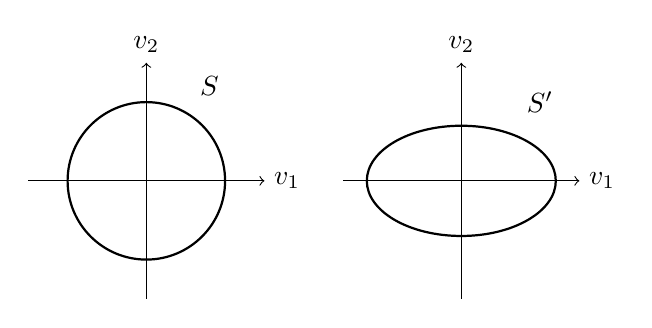
\begin{tikzpicture}[scale=1.0]
            \draw[->] (-1.5,0) -- (1.5,0) node[right] {$v_1$};
            \draw[->] (0,-1.5) -- (0,1.5) node[above] {$v_2$};
            \draw[thick] (0,0) circle (1);
            \node at (0.8, 1.2) {$S$};
            
            \begin{scope}[xshift=4cm]
                \draw[->] (-1.5,0) -- (1.5,0) node[right] {$v_1$};
                \draw[->] (0,-1.5) -- (0,1.5) node[above] {$v_2$};
                \draw[thick] (0,0) ellipse (1.2 and 0.7);
                \node at (1.0, 1.0) {$S'$};
            \end{scope}
        \end{tikzpicture}
    \end{center}
\end{example}

\begin{example}
    Let $A = \begin{pmatrix} 1 & -1 \\ -1 & 2 \end{pmatrix}$. It is positive definite (why?). Let $\langle \cdot, \cdot \rangle :=$ std. scalar prod, and $\langle \cdot, \cdot \rangle' := \langle \cdot, \cdot \rangle_A$.
    We have:
    \[
        \left\langle \begin{pmatrix} 1 \\ 0 \end{pmatrix}, \begin{pmatrix} 1 \\ 1 \end{pmatrix} \right\rangle = 1, \quad \left\langle \begin{pmatrix} 1 \\ 0 \end{pmatrix}, \begin{pmatrix} 1 \\ 1 \end{pmatrix} \right\rangle' = \begin{pmatrix} 1 & 0 \end{pmatrix} \cdot \begin{pmatrix} 1 & -1 \\ -1 & 2 \end{pmatrix} \begin{pmatrix} 1 \\ 1 \end{pmatrix} = \begin{pmatrix} 1 & -1 \end{pmatrix} \begin{pmatrix} 1 \\ 1 \end{pmatrix} = 0.
    \]
    So $\left(\begin{smallmatrix} 1 \\ 0 \end{smallmatrix}\right) \perp' \left(\begin{smallmatrix} 1 \\ 1 \end{smallmatrix}\right)$ but $\left(\begin{smallmatrix} 1 \\ 0 \end{smallmatrix}\right) \not\perp \left(\begin{smallmatrix} 1 \\ 1 \end{smallmatrix}\right)$.
\end{example}

\subsection*{A different type of example}

Let $C[a,b] =$ space of continuous functions $f: [a,b] \to \mathbb{R}$. It is a vector space over $\mathbb{R}$ with respect to the standard operations. 
We define a scalar product:
\[
    \langle f, g \rangle := \int_a^b f(x) \cdot g(x) \, dx.
\]
(This is well-defined and finite. Why?)

\begin{exercise}
    Show that $\langle \cdot, \cdot \rangle$ is linear in both variables and symmetric.
\end{exercise}

Let's check positivity: let $0 \neq f \in C[a,b]$. Then $\langle f, f \rangle = \int_a^b f(x)^2 \, dx$. Since $f \neq 0$, there exists $x_0 \in (a,b)$ such that $f(x_0) \neq 0$. Since $f$ is continuous, so is $f^2$. Hence, there exists $\delta > 0$ such that $[x_0 - \delta, x_0 + \delta] \subseteq [a,b]$ and $f(x) \neq 0$ for all $x \in [x_0 - \delta, x_0 + \delta]$. This implies $f(x)^2 > 0$ for all $x \in [x_0 - \delta, x_0 + \delta]$. Therefore,
\[
    \langle f, f \rangle = \int_a^b f(x)^2 \, dx \geq \int_{x_0 - \delta}^{x_0 + \delta} f(x)^2 \, dx \geq 2\delta \cdot \min_{x \in [x_0-\delta, x_0+\delta]} f(x)^2 > 0.
\]

\begin{remark}
    By this scalar product on $C[-\pi, \pi]$, the functions $f(x) = \sin x$ and $g(x) \equiv 1$ are orthogonal ($f \perp g$).
\end{remark}

\subsection*{Norms and angles}

% Def. (22.a.10)
\begin{definition}
\label{def:norm}
    Let $V$ be a vector space over $K$ (where $K = \mathbb{R}$ or $\mathbb{C}$). A \newterm{norm} on $V$ is a function $\| \cdot \|: V \to \mathbb{R}_{\geq 0}$ such that:
    \begin{enumerate}[label=\textbf{(\alph*)}]
        \item $\|u + v\| \leq \|u\| + \|v\|$ for all $u, v \in V$. (Triangle inequality)
        \item $\|\alpha \cdot v\| = |\alpha| \cdot \|v\|$ for all $\alpha \in K, \; v \in V$. (Homogeneity)
        \item If $\|v\| = 0$, then $v = 0$. (Non-degeneracy)
    \end{enumerate}
    
    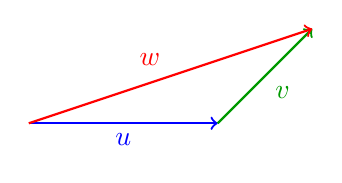
\begin{tikzpicture}[baseline=(current bounding box.center), scale=1.2]
        \draw[->, blue, thick] (0,0) -- (2,0) node[midway, below] {$u$};
        \draw[->, green!60!black, thick] (2,0) -- (3,1) node[midway, below right] {$v$};
        \draw[->, red, thick] (0,0) -- (3,1) node[midway, above left] {$w$};
    \end{tikzpicture}
\end{definition}

\begin{claim*}
    If $\langle \cdot, \cdot \rangle$ is an inner product on $V$, then $\|v\| := \sqrt{\langle v, v \rangle}$ is a norm on $V$. (We'll prove this soon).
\end{claim*}

\begin{exercise}
    Define $\left\| \binom{a}{b} \right\|' := \max\{|a|, |b|\}$, and $\left\| \binom{a}{b} \right\|'' := |a| + |b|$ for all $\binom{a}{b} \in \mathbb{R}^2$. Show that $\| \cdot \|'$ and $\| \cdot \|''$ are norms, but they are not induced by any scalar product. 
    
    \textit{Hint:} Recall that if the scalar product $\langle \cdot, \cdot \rangle$ induces $\| \cdot \|$, then $\langle u, v \rangle = \frac{1}{2} (\|u + v\|^2 - \|u\|^2 - \|v\|^2)$.
\end{exercise}

% Thm. (22.a.11)
\begin{theorem}[Cauchy-Schwarz Inequality]
\label{thm:cauchy_schwarz}
    Let $(V, \langle \cdot, \cdot \rangle)$ be a vector space endowed with an inner product $\langle \cdot, \cdot \rangle$. Then for all $u, v \in V$ we have 
    \[
        |\langle u, v \rangle| \leq \|u\| \cdot \|v\|,
    \]
    with equality if and only if $u$ and $v$ are proportional (i.e., $u = \alpha \cdot v$, or $v = \alpha \cdot u$ for some $\alpha \in K \iff u, v$ are linearly dependent).
\end{theorem}

\begin{proof}
    If $u = 0$, the (in)equality holds, so assume $u \neq 0$. 
    Put $w := v - \lambda \cdot u$, where $\lambda := \frac{\langle v, u \rangle}{\|u\|^2}$. (*)
    
    We have $\langle w, u \rangle = \langle v, u \rangle - \lambda \langle u, u \rangle = 0$.
    Now:
    \begin{align*}
        0 &\leq \|w\|^2 = \langle v - \lambda u, v - \lambda u \rangle \\
        &= \langle v, v \rangle - \overline{\lambda} \langle v, u \rangle - \lambda \langle u, v \rangle + \lambda \overline{\lambda} \langle u, u \rangle \\
        &= \|v\|^2 - \overline{\lambda} \cdot \lambda \|u\|^2 - \lambda \cdot \overline{\lambda} \|u\|^2 + \lambda \cdot \overline{\lambda} \|u\|^2 \quad \left(\text{since } \overline{\langle v, u \rangle} = \overline{\lambda} \|u\|^2 \text{ and } \langle u, v \rangle = \lambda \|u\|^2\right) \\
        &= \|v\|^2 - |\lambda|^2 \|u\|^2 \\
        &= \|v\|^2 - \frac{|\langle v, u \rangle|^2}{\|u\|^4} \cdot \|u\|^2 \\
        &= \|v\|^2 - \frac{|\langle v, u \rangle|^2}{\|u\|^2}.
    \end{align*}
    This implies $0 \leq \|v\|^2 - \frac{|\langle v, u \rangle|^2}{\|u\|^2}$, which implies $|\langle v, u \rangle| \leq \|u\| \cdot \|v\|$.
    
    We have equality if and only if either $u = 0$, or $w = 0$.
    But $w = 0 \iff v = \lambda u$ where $\lambda = \frac{\langle v, u \rangle}{\|u\|^2}$.
    But for $u \neq 0$, the condition $v = \lambda u$ implies $\lambda = \frac{\langle v, u \rangle}{\|u\|^2}$.
    So, equality if and only if either $u = 0$ or $v = \lambda u$ for some $\lambda \in K \iff u, v$ are linearly dependent.
\end{proof}

% Cor. (22.a.12)
\begin{corollary}
\label{cor:norm_induced}
    Let $V$ be a vector space and $\langle \cdot, \cdot \rangle$ an inner product on $V$. Then $V \ni v \mapsto \|v\| := \sqrt{\langle v, v \rangle}$ is a norm on $V$.
\end{corollary}

\begin{proof}
    We assume $(V, \langle \cdot, \cdot \rangle)$ is a Hermitian space (the case of Euclidean space is very similar).
    
    \underline{Triangle inequality:} Let $u, v \in V$.
    \begin{align*}
        \|u + v\|^2 &= \langle u + v, u + v \rangle = \langle u, u \rangle + \langle u, v \rangle + \langle v, u \rangle + \langle v, v \rangle \\
        &= \|u\|^2 + 2 \operatorname{Re} \langle u, v \rangle + \|v\|^2. \quad (*)
    \end{align*}
    Note that for all $z \in \mathbb{C}$ we have $|\operatorname{Re} z| \leq |z|$. (Indeed, if $z = x + iy$, $x, y \in \mathbb{R}$, then $|\operatorname{Re} z| = |x| \leq \sqrt{x^2 + y^2} = |z|$).
    Applying this to our situation, we have $\operatorname{Re} \langle u, v \rangle \leq |\operatorname{Re} \langle u, v \rangle| \leq |\langle u, v \rangle|$.
    Going back to (*), we get:
    \[
        \|u + v\|^2 \leq \|u\|^2 + 2 |\langle u, v \rangle| + \|v\|^2 \leq \|u\|^2 + 2 \|u\| \cdot \|v\| + \|v\|^2 = (\|u\| + \|v\|)^2,
    \]
    where the second inequality follows from the Cauchy-Schwarz inequality.
    Since both $\|u + v\|$ and $\|u\| + \|v\|$ are non-negative, the last inequality implies that $\|u + v\| \leq \|u\| + \|v\|$.
    
    The other properties of being a norm: Exercise.
\end{proof}

% Def. (22.a.13)
\begin{definition}
\label{def:angle}
    Let $(V, \langle \cdot, \cdot \rangle)$ be a Euclidean space. Let $u, v \in V$ be two non-zero vectors. By the Cauchy-Schwarz inequality, $-1 \leq \frac{\langle u, v \rangle}{\|u\| \cdot \|v\|} \leq 1$. We define the \newterm{angle} between $u$ and $v$ to be the unique $\alpha \in [0, \pi]$ such that:
    \[
        \cos \alpha = \frac{\langle u, v \rangle}{\|u\| \cdot \|v\|} \quad \left(= \left\langle \frac{u}{\|u\|}, \frac{v}{\|v\|} \right\rangle\right).
    \]
    \begin{center}
        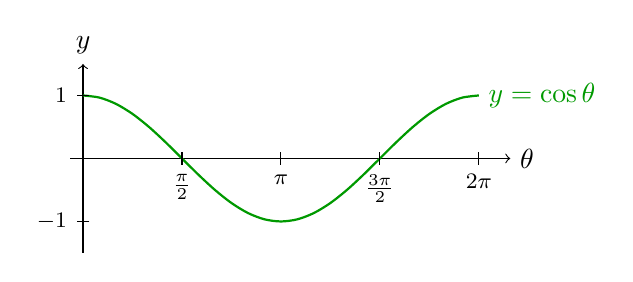
\begin{tikzpicture}[scale=0.8]
            \draw[->] (-0.2,0) -- (2*pi+0.5,0) node[right] {$\theta$};
            \draw[->] (0,-1.5) -- (0,1.5) node[above] {$y$};
            \draw[domain=0:2*pi, smooth, variable=\x, green!60!black, thick] plot ({\x}, {cos(\x*180/pi)});
            \node[green!60!black, right] at (2*pi, 1) {$y = \cos \theta$};
            
            \draw (pi/2, 0.1) -- (pi/2, -0.1) node[below] {\footnotesize $\frac{\pi}{2}$};
            \draw (pi, 0.1) -- (pi, -0.1) node[below] {\footnotesize $\pi$};
            \draw (3*pi/2, 0.1) -- (3*pi/2, -0.1) node[below] {\footnotesize $\frac{3\pi}{2}$};
            \draw (2*pi, 0.1) -- (2*pi, -0.1) node[below] {\footnotesize $2\pi$};
            
            \draw (0.1, 1) -- (-0.1, 1) node[left] {\footnotesize $1$};
            \draw (0.1, -1) -- (-0.1, -1) node[left] {\footnotesize $-1$};
        \end{tikzpicture}
    \end{center}
\end{definition}

\subsection*{The Gram-Schmidt orthogonalization process.}

% Thm. (22.a.14)
\begin{theorem}
\label{thm:properties_orthogonal_systems}
    Let $(V, \langle \cdot, \cdot \rangle)$ be an inner product space.
    \begin{enumerate}[label=\textbf{(\alph*)}]
        \item If $S \subseteq V$ is an orthogonal system, then $S$ is linearly independent.
        \item If $v_1, \dots, v_n$ is an orthogonal system and $v \in \Sp(v_1, \dots, v_n)$, write $v = a_1 v_1 + \dots + a_n v_n$, with $a_j \in K$ (where $K = \mathbb{R}$ or $\mathbb{C}$). Then the coefficients $a_j$ are given by 
        \[
            a_j = \frac{\langle v, v_j \rangle}{\langle v_j, v_j \rangle} \quad \forall \; 1 \leq j \leq n.
        \]
    \end{enumerate}
\end{theorem}

\begin{proof}
    \textbf{(b)} Write $v = a_1 v_1 + \dots + a_n v_n$. Let $1 \leq j \leq n$. We have:
    \[
        \langle v, v_j \rangle = \sum_{k=1}^n a_k \underbrace{\langle v_k, v_j \rangle}_{= 0 \; \forall k \neq j} = a_j \langle v_j, v_j \rangle,
    \]
    which implies that
    \[
        a_j = \frac{\langle v, v_j \rangle}{\langle v_j, v_j \rangle}.
    \]
    
    \textbf{(a)} Suppose $\sum_{k=1}^n a_k v_k = 0$, where $n \geq 1$, $v_1, \dots, v_n \in S$ are distinct and $a_1, \dots, a_n \in K$. By \textbf{(b)},
    \[
        a_j = \frac{\langle 0, v_j \rangle}{\langle v_j, v_j \rangle} = 0 \quad \forall \; 1 \leq j \leq n.
    \]
\end{proof}

% Prop. (22.a.15)
\begin{proposition}
\label{prop:matrix_representation_orthonormal}
    Let $V, W$ be vector spaces over $K$ ($= \mathbb{R}$ or $\mathbb{C}$) and let $\langle \cdot, \cdot \rangle$ be an inner product on $W$. Let $\mathcal{B} = (v_1, \dots, v_n)$ be a basis for $V$ and $\mathcal{C} = (w_1, \dots, w_m)$ an \emph{orthonormal} basis for $W$. Let $T: V \to W$ be a linear map. Write $[T]_{\mathcal{C}}^{\mathcal{B}} = (a_{ij})$. Then $a_{ij} = \langle T(v_j), w_i \rangle$ for all $i,j$. 
    (If $\mathcal{C}$ is only an orthogonal basis, then $a_{ij} = \langle T(v_j), w_i \rangle / \langle w_i, w_i \rangle$).
\end{proposition}

\begin{proof}
    Exercise.
\end{proof}

So, having orthogonal/orthonormal bases for our spaces is useful!

% Thm. (22.a.16)
\begin{theorem}[Gram-Schmidt orthogonalization process]
\label{thm:gram_schmidt}
    Let $(V, \langle \cdot, \cdot \rangle)$ be an inner product space over $K$ ($= \mathbb{R}$ or $\mathbb{C}$) and let $n = \dim V$. Let $(v_1, \dots, v_n)$ be a basis of $V$. Define a new list of vectors $w_1, \dots, w_n$ by induction:
    \[
        w_1 := v_1, \quad w_j := v_j - \sum_{i=1}^{j-1} \frac{\langle v_j, w_i \rangle}{\langle w_i, w_i \rangle} \cdot w_i \quad \text{for } j = 2, \dots, n.
    \]
    Then:
    \begin{enumerate}[label=\textbf{(\alph*)}]
        \item $(w_1, \dots, w_n)$ is an orthogonal basis for $V$.
        \item $\left( \frac{w_1}{\|w_1\|}, \dots, \frac{w_n}{\|w_n\|} \right)$ is an orthonormal basis for $V$.
        \item $\forall \; 1 \leq j \leq n$ we have $\Sp(v_1, \dots, v_j) = \Sp(w_1, \dots, w_j) = \Sp\left(\frac{w_1}{\|w_1\|}, \dots, \frac{w_j}{\|w_j\|}\right)$.
    \end{enumerate}
\end{theorem}

\begin{proof}
    We claim that for all $1 \leq j \leq n$, $w_j$ is well defined (i.e., $w_1, \dots, w_{j-1} \neq 0$, recall that we need to divide by $\langle w_i, w_i \rangle$ in $i = 1, \dots, j-1$ in order to define $w_j$), and moreover $(w_1, \dots, w_j)$ is an orthogonal system with $\Sp(w_1, \dots, w_j) = \Sp(v_1, \dots, v_j)$.
    
    We prove this by induction on $j$.
    
    For $j = 1$, $w_1 = v_1$, so the claim is obvious ($v_1 \neq 0$ because it is a part of a basis).
    
    Let $2 \leq j \leq n$. Assume the claim holds for $w_1, \dots, w_{j-1}$.
    Recall that $w_j = v_j - \sum_{i=1}^{j-1} \frac{\langle v_j, w_i \rangle}{\langle w_i, w_i \rangle} \cdot w_i$. Note that $w_j$ is well defined because $w_i \neq 0$ for all $1 \leq i \leq j-1$. We claim that $w_j \neq 0$. Indeed, if $w_j = 0$, then 
    \[
        v_j = \sum_{i=1}^{j-1} \frac{\langle v_j, w_i \rangle}{\langle w_i, w_i \rangle} w_i \implies v_j \in \Sp(w_1, \dots, w_{j-1}) = \Sp(v_1, \dots, v_{j-1})
    \]
    (by inductive hypothesis), which is impossible because $(v_1, \dots, v_j)$ are linearly independent.
    
    This shows $w_j \neq 0$. By the inductive hypothesis, $w_1, \dots, w_{j-1}$ is an orthogonal system. So we have to prove that $w_j \perp w_1, \dots, w_{j-1}$.
    Indeed, let $1 \leq k \leq j-1$. Then
    \[
        \langle w_j, w_k \rangle = \langle v_j, w_k \rangle - \sum_{i=1}^{j-1} \frac{\langle v_j, w_i \rangle}{\langle w_i, w_i \rangle} \cdot \langle w_i, w_k \rangle = \langle v_j, w_k \rangle - \frac{\langle v_j, w_k \rangle}{\langle w_k, w_k \rangle} \cdot \langle w_k, w_k \rangle = 0.
    \]
    This shows $(w_1, \dots, w_j)$ is an orthogonal system. 
    
    To complete the induction, it remains to show that $\Sp(w_1, \dots, w_j) = \Sp(v_1, \dots, v_j)$. By the definition of $w_j$ we have
    \[
        w_j \in \Sp(w_1, \dots, w_{j-1}, v_j) = \Sp(v_1, \dots, v_{j-1}, v_j) \quad \text{(inductive hypothesis)}.
    \]
    This implies $\Sp(w_1, \dots, w_{j-1}, w_j) \subseteq \Sp(v_1, \dots, v_{j-1}, v_j)$. But both these vector spaces have dimension $j$ (because $v_1, \dots, v_j$ are linearly independent, and also $w_1, \dots, w_j$ are linearly independent, being an orthogonal system). This implies $\Sp(w_1, \dots, w_{j-1}, w_j) = \Sp(v_1, \dots, v_{j-1}, v_j)$.
\end{proof}

% Cor. (22.a.17)
\begin{corollary}
\label{cor:orthonormal_basis_exists}
    Every finite-di\-men\-sional inner product space has an orthonormal basis.
\end{corollary}

Geometric idea behind the Gram-Schmidt process.
\begin{center}
    \begin{tikzpicture}[scale=1.2]
        % Plane W_{j-1}
        \fill[green!20] (-2,-1) -- (2,-1) -- (3,1) -- (-1,1) -- cycle;
        \draw (-2,-1) -- (2,-1) -- (3,1) -- (-1,1) -- cycle;

        % Label of plane
        \node at (-1.5,-0.7) {$W_{j-1}$};

        % Origin
        \coordinate (O) at (0,0);
        \fill (O) circle (1.2pt) node[left] {$0$};

        % Projection point
        \coordinate (P) at (1.1,0.2);
        \fill (P) circle (1.2pt);
        \node[below, yshift=-2pt] at (P) {$\Pr(v_j)$};

        % v_j vector
        \coordinate (V) at (1.6,2.3);
        \draw[->, thick] (O) -- (V);
        \node[left] at ($(O)!0.6!(V)$) {$v_j$};

        % w_j vector
        \draw[->, thick] (P) -- (V);
        \node[right] at ($(P)!0.5!(V)$) {$w_j = v_j - \Pr_{W_{j-1}}(v_j)$};

        % projection vector
        \draw[->, thick] (O) -- (P);

        % dashed orthogonal drop
        \draw[dashed] (V) -- (P);

        % right angle marker
        \draw ($(P)+(0.12,0)$) -- ($(P)+(0.12,0.12)$) -- ($(P)+(0,0.12)$);

        % Span text
        \node[right] at (1, -0.4) {$\Sp(v_1,\dots,v_{j-1})=\Sp(w_1,\dots,w_{j-1}) := W_{j-1}$};

        % Formula (like in sketch)
        \node[right] at (2.5, 2.0) {$(v_j = w_j + \Pr_{W_{j-1}}(v_j))$};

    \end{tikzpicture}
\end{center}

Orthogonal projection:
\[
    \Pr_{W_{j-1}}(v_j) = \sum_{i=1}^{j-1} \frac{\langle v_j, w_i \rangle}{\langle w_i, w_i \rangle} \cdot w_i.
\]
We'll see more about this soon.

\vspace{2em}

\subsection*{Solutions to Exercises}

\begin{exercisesolution}[Proof of Polarization Identity (on \cpageref{exc:reconstruct_scalar_prod} \textbf{(b)})]
    Let $V$ be a Hermitian space. The analogous formula to reconstruct the Hermitian product from the norm is the Polarization Identity:
    \[
        \langle u, v \rangle = \frac{1}{4}\left(\|u+v\|^2 - \|u-v\|^2 + i\|u+iv\|^2 - i\|u-iv\|^2\right).
    \]
    By expanding each norm term using $\|x+y\|^2 = \|x\|^2 + \|y\|^2 + 2\operatorname{Re}\langle x, y \rangle$ and maintaining careful track of the imaginary components through sesquilinearity, the cross terms isolate $\langle u, v \rangle$.
\end{exercisesolution}

\begin{exercisesolution}[Positive Definite Matrices (on \cpageref{exc:pos_def_2x2_complex})]
    Let $A = \begin{pmatrix} a & b \\ \overline{b} & d \end{pmatrix} \in \M_{2 \times 2}(\mathbb{C})$ be a Hermitian matrix (which implies $a, d \in \mathbb{R}$). 
    For $v = (x, y)^\top \in \mathbb{C}^2$, the condition $v^\top A \overline{v} > 0$ yields
    \[
        a|x|^2 + b x \overline{y} + \overline{b} \overline{x} y + d|y|^2 > 0.
    \]
    Choosing $v = (1, 0)^\top$ gives $a > 0$. Through completing the square, the full expression is positive for all non-zero $v$ if and only if $a > 0$ and $ad - |b|^2 > 0$. This confirms the condition $a > 0$ and $\det A > 0$.
\end{exercisesolution}